\chapter{Le stockage d'énergie par air comprimé}

\section{Introduction}

Afin de conserver l'énergie électrique non utilisée en heure creuse, le stockage par air comprimé est une solution envisageable. Actuellement, il existe deux systèmes en fonctionnement, un à Huntorf en Allemagne et l'autre à Mcintosh Alabama aux États-Unis.\\

La démarche global consiste à utiliser l'électricité pour activer des compresseurs qui comprimerons l'air ambiant pour ensuite le stocker dans une cave en sous-sol. Il y a alors transformation de l'énergie électrique en énergie mécanique. Cependant, lors de cette compression, il y a échauffement de l'air. Hors, cette énergie est perdue vers le milieu extérieur. L'objectif est donc de récupérer celle-ci grâce à un stockage de chaleur sensible. Par conséquent, nous allons dimensionner ce stockage pour la centrale de Huntorf. \\

Dans un premier temps, nous allons décrire le système. Puis nous ferons un rapide bilan thermodynamique pour vérifier si le stockage de chaleur sensible possède un intérêt. Enfin, nous réaliserons une petite analyse économique afin de quantifier les gains possibles et donc l'investissement réalisable pour construire cette installation.
\newpage

\section{Description du principe général}

\subsection{Le cycle de l'air}

\begin{figure}[!h]
\centering

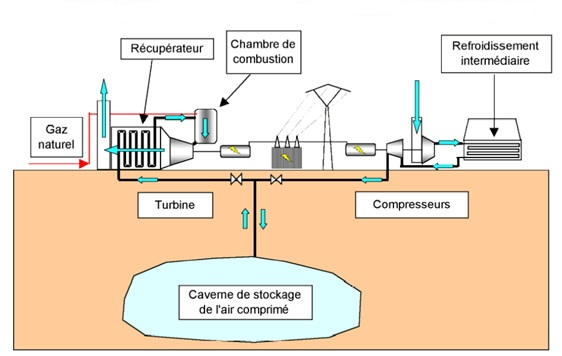
\includegraphics[scale=0.7]{PHOTO/shema_base.jpg}
\label{sh_base}
\caption{Schéma d'un stockage d'énergie par air comprimé}
\end{figure}

Comme nous pouvons le visualiser sur la figure \ref{sh_base}, l'air est comprimé par un compresseur en heure creuse. Lors de cette étape, l'air va être fortement réchauffé. Il va donc être refroidis par un échangeur classique. Ainsi fait, il va être stocké dans une caverne naturelle sous haute pression.\\


Lorsque l'on va passer en heure pleine, il va être déstocké et réchauffé par du gaz naturelle dans une chambre à combustion, notamment pour éviter que l'eau contenue dans l'air ne se condense. Cette étape est crucial puisque l'air va ensuite être détendu dans une turbine. Dans ces circonstances, il faut empêcher tous risques de cavitation, et donc d'eau sous forme liquide, pour éviter une usure prématuré de la turbine. Pour finir le cycle, la rotation de la turbine, relié à un alternateur, va produire de l'énergie sous forme électrique. Ainsi, celle ci va pouvoir être distribuée par le réseau électrique.\\


Comme nous souhaitons récupérer l'énergie perdue lors de la compression, nous allons regarder plus en détail le système "compresseur".

\subsection{La compression}
 
 Sur la figure \ref{sh_fonc}, nous remarquons la présence de trois compresseurs : basse, moyenne et haute pression. 
 
Les étages de compressions sont réalisés pour deux raisons. La plus importante est que la compression de l'air entraine une augmentation de la température du gaz. Hors, la dilatation des matériaux, provoquée par la chaleur, peut entrainer la destruction du compresseur. La solution consiste donc à refroidir les gaz, par un échangeur, entre plusieurs étages de compressions. 

L'autre raison est qu'il existe plusieurs technologies de compresseurs ce qui a pour conséquence d'avoir des coûts et rendements différents. Nous allons décrire rapidement les trois types de compresseurs utilisés dans le stockage d'air comprimé.

\subsubsection{Compresseur piston}

Le principe est relativement simple. Un piston est mis en mouvement pour comprimé l'air. Il existe des systèmes qui permettent de comprimer l'air au-dessus et en-dessous du piston. L'on peut ensuite aligner plusieurs cylindres pour atteindre de très hautes pressions.

Ces pistons permettent de d'augmenter la pressions entre 1.5 et 414 bar pour un travaille fourni comprit entre 0.75kW et 420kW.
 
\subsubsection{Compresseur à vis}

 C'est le système le plus utilisé. Chaque éléments possèdent un rotor mâle et femelle se déplacent l'un dans l'autre, provoquant ainsi une diminution du volume et donc une augmentation de pression.  
 
Il produit une élévation de pression de 5 à 13 bar pour un travaille comprit entre 4kW et 250kW.

\subsubsection{compresseur à palettes}
 
 Un rotor, possédant un certains nombres de fentes, est mis en rotation. Dans chaque fentes est inséré une palette qui par force centrifuge se déplace vers les parois provoquant ainsi la compression du gaz. La chaleur dégagé lors de la compression est contrôlé par injection d'huile.
 
 Ces pistons permettent de d'augmenter la pressions de 7 à 10 bar pour un travaille fourni comprit entre 1.1kW et 75kW.\\
 
 Ayant étudié le système, nous allons estimer la chaleur perdu par compression et la chaleur fournie par combustion.
 
\section{Calcule de l'énergie perdue et nécessaire par le système}

Il est estimé que si l'on pouvais récupérer la chaleur dégagé lors de la compression, l'on pourrai réduire la consommation de gaz naturel de 25\%. Pour l'usine de Huntorf, 5600kJ de gaz naturel pour 1Kwh d'énergie en sortie est nécessaire. L'objectif de cette partie va être de comparer la chaleur produite par compression et par combustion pour vérifier si il est pertinent de dimensionner un stockage de chaleur sensible.


\subsection{Calcule de la chaleur perdue}

Nous allons estimer, par les principes thermodynamiques, la chaleur dégagée par la compression. 

Celui ci est établie à partir des données visualisables sur la figure \ref{sh_fonc} et du tableau \ref{tab1}.\\


\begin{figure}[!h]
\centering
\caption{Schéma de la centrale de Mcintosh avec certaines grandeurs thermos-physiques}
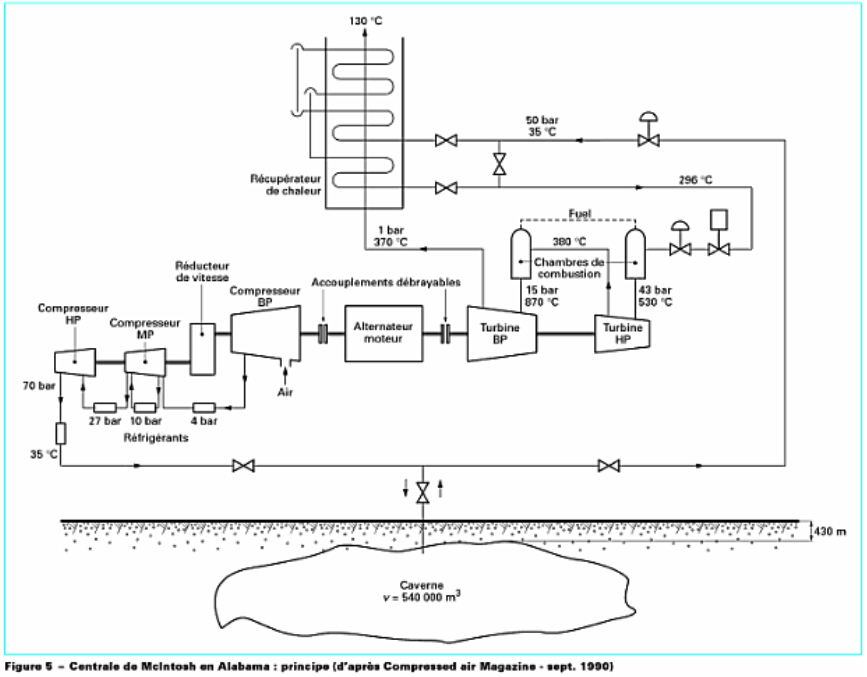
\includegraphics[scale=0.5]{PHOTO/shema_fonctionnement.jpg}
\label{sh_fonc}
\end{figure}


\begin{figure}[!h]
\centering
\caption{Tableau regroupant certaines données de la centrale de Huntorf}
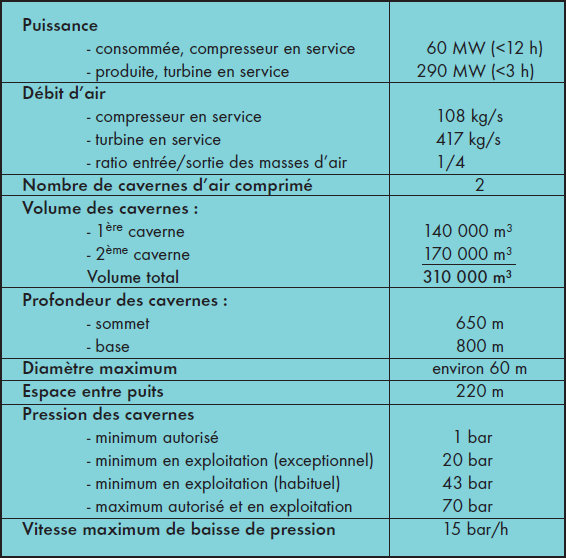
\includegraphics[scale=0.5]{PHOTO/tab1.png}
\label{tab1}
\end{figure}






\newpage

Puisqu'il nous manque un certain nombres de données, nous supposerons une compression avec un rendement isentropique de 80\%. L'air extérieur sera considéré comme étant à 300 Kelvin et à 1 Atmosphère. Nous considérons que la pression de sortie des compresseurs est de 70 Bar.\\

Nous calculons l'état de l'air après une compression isentropique. Cela nous permet d'écrire la formule suivante : 

\begin{equation}
Pr(T2)=Pr(T1)\frac{P2}{P1}
\label{pr_is}
\end{equation}

A l'état initial nous avons :

\begin{itemize}
\item T1=300K
\item P1=1atm
\item Pr(T1)=1,386
\item h1=300,19 kJ/kg\\
\end{itemize}

Donc à l'état final nous obtenons à partir de l'équation \ref{pr_is} et des tables de l'air :
 
\begin{itemize}
\item P2=70bar
\item Pr(T2)=97,0
\item h2=1000,55 kJ/kg
\item T2=960K\\

\end{itemize}

Avec un rendement isentropique ($\eta$) de 80\% nous avons l'équation \ref{rd_is}.

\begin{equation}
h3=\frac{h2-h1}{\eta}+h1
\label{rd_is}
\end{equation}

Ainsi, nous déterminons l'état "réel" 3 :

\begin{itemize}
\item h3=1175,64 kJ/kg
\item T3=1112,5 K\\

\end{itemize}



En sortie, les données nous disent que l'air à une température T4 de 310K. Ce qui nous donne une enthalpie h4 de 310,24 kJ/kg. De plus, on sait que le débit d'air est de 108 kg/s.
En considérant une transformation isobare et en appliquant le premier principe nous obtenons l'énergie récupérable :

\begin{equation}
Q=\dot{m}(h4-h3) = -93463.2 kW
\label{cha_recup}
\end{equation}


Nous regardons combien de kilogramme d'air sont stockées dans la caverne. L'objectif est de faire un bilan complet sur un cycle de stockage. 
Avec l'équation des gaz parfaits, nous obtenons la masse volumique de l'air à 70 bar et 310K (equation \ref{mv}). 

\begin{equation}
v4=\frac{P4}{T4*r}=80,00 kg/m^{3}
\label{mv}
\end{equation}

Avec $r=\frac{R}{M_{air}}=282,29 kg/m^{3}$\\


Nous faisons l'hypothèse que la température de l'air est constante pour une valeur de 310K.

Les cavernes de Huntorf ont un volume total de $310.000 m^{3}$. Nous pouvons donc stocker $2,48000.10^{7} kg$. Cependant, en pression, le minimum opérationnel des cavernes est de 43 bar. La masse volumique à cette pression est $v=49,14kg/m^{3}$. Donc on ne peut déstocker $1,52326.10^{7} kg$. Ce qui nous fait, au final, une masse utilisable de $m=0,95674.10^{7} kg$. \\

En reprenant le débit des compresseurs, nous remplissons la caverne en 92592 secondes. Nous obtenons donc pour un cycle de stockage $8,654.10^{9} kJ$ soit $2403,8 MWh$.\\
\newpage

\subsection{Calcule de la chaleur de combustion}

Nous allons estimer l'énergie nécessaire par combustion.

En entrée, nous avons un fluide qui arrive à 43 bar et 570K (état 5). Il est ensuite réchauffé à 803K dans une chambre de combustion (état 6). Nous regardons qu'elle est l'énergie qu'on a dû lui fournir pour une transformation isobare. \\


Nous avons donc :

\begin{itemize}
\item T5=570K
\item h5=575,59kJ/kg\\

\item T6=803K
\item P6=43bar
\item h6=825,25kJ/kg\\

\end{itemize}

Soit $Q_{combustion,1}=m(h6-h5)=663,5MWh$\\


Le passage dans la turbine provoque une détente qui fait passer le gaz à l'état 7 pour ensuite être réchauffé par une nouvelle combustion qui fait passer l'air à l'état 8.

\begin{itemize}
\item T7=650K
\item h7=659,84kJ/kg\\

\item T8=1140K
\item h8=1207,57kJ/kg\\

\end{itemize}

Soit $Q_{combustion,2}=m(h8-h7)=1455.6MWh$\\


Ce qui nous fait le total d'énergie de combustion nécessaire suivant :

 $Q_{total}=Q_{combustion,1}+Q_{combustion,2}=2118,5MWh$.\\

Au final, Nous pouvons remarquer que l'énergie perdue lors de la compression est supérieur à l'énergie nécessaire lors des combustions. Donc dans l'absolue, nous pouvons penser que si nous arrivons à stocker cette énergie de compression, nous pouvons supprimer l'utilisation de gaz naturel.\\

 Cependant, le manque d'information sur le système et en particulier sur le rendement des compresseurs ne permet pas d'avoir une quantification exacte de la réalité. Ce calcule nous donne seulement un ordre de grandeur mais permet tout de même de vérifier la pertinence de dimensionner un stockage de chaleur. De plus, la présence de gaz à très haute température permet de chauffer notre stockage de chaleur sensible aux alentours de 1000 Kelvin; ce qui permet par la suite de monter la température de notre air à celle souhaité tout en respectant le second principe.


\section{Analyse économique}

En France, le tarif réglementé du gaz naturelle s'élève à 0,0580 \euro TTC/kWh. Donc si nous occultons les rendements de la combustion, nous avons un coût en gaz naturelle de 122.873 euros pour un cycle de stockage. Si nous estimons un cycle par jour, nous avons un coût annuelle de 44.234.280 euros. Si nous imaginons que le stockage permet d'économiser 25\% de gaz naturelle, nous avons une économie annuelle de 11.058.570 euros. Supposons que l'on souhaite amortir l'investissement du stockage en 3ans, nous avons 33.175.710 euros disponible pour le réaliser. \\

En conclusion, nous pouvons clairement affirmer que ce stockage permet de réaliser un gain substantif rapidement.












